\documentclass[11pt]{article}
\usepackage[T1]{fontenc}
\usepackage[utf8]{inputenc}
\usepackage{lmodern}
\usepackage[a4paper,margin=1in]{geometry}
\usepackage{amsmath,amssymb,amsthm,amscd,mathtools}
\usepackage{tikz}
\usepackage{microtype}
\usepackage[hidelinks]{hyperref}
\hypersetup{pdftitle={Étale covers with a prescribed exterior sheet},pdfauthor={OpenAI}}
\usepackage{enumitem}
\numberwithin{equation}{section}
\newtheorem{theorem}{Theorem}[section]
\newtheorem{proposition}[theorem]{Proposition}
\newtheorem{lemma}[theorem]{Lemma}
\theoremstyle{remark}
\newtheorem{remark}[theorem]{Remark}
\DeclareMathOperator{\Gal}{Gal}
\title{\'{E}tale covers with a prescribed exterior sheet}
\author{OpenAI}
\date{September 24, 2026}
\pdfinfoomitdate=1
\pdftrailerid{}
\pdfsuppressptexinfo=15
\begin{document}
\maketitle
\begin{abstract}
Let $X$ be a smooth proper hyperbolic curve over an algebraic closure
of a $p$-adic local field. Given finitely many disjoint small open disks,
we construct one connected finite \'etale cover with a sheet isomorphic
to their entire exterior and with degree divisible by $p$ on every
connected component above each disk.
\end{abstract}

\tableofcontents

\section{The simultaneous covering statement}

Fix a prime $p$, a finite extension $k/\mathbb Q_p$, an algebraic
closure $\bar k$, and its completion $\Omega=\widehat{\bar k}$.
All analytic spaces below are Berkovich spaces over $\Omega$.
For a curve $X/\bar k$ write $X^{\rm an}=(X_\Omega)^{\rm an}$.
The additive valuation is normalized by $v(p)=1$, so that
$v(\Omega^\times)=\mathbb Q$.

Let $X/\bar k$ be smooth, proper and connected, of genus at least two.
Choose distinct points $b_1,\ldots,b_d\in X(\bar k)$, where $d\ge1$,
and rational local parameters $t_i$ at these points. Suppose there
are pairwise disjoint open disks $B_i\subset X^{\rm an}$ on which
$t_i$ identifies $B_i$ with $\{|T|<R_i\}$, and radii
$r_i\in|\Omega^\times|$ with $0<r_i<R_i$. Set
\[
 V_i=\{x\in B_i:|t_i(x)|<r_i\}.
\]
Thus the closed disk of radius $r_i$ lies strictly inside its parameter
chart. Put
\[
 U=X^{\rm an}\setminus\bigcup_{i=1}^d V_i,
\]
and suppose that $U$ is nonempty and contains an $\Omega$-rational
point. It is a compact connected analytic domain: removing each open
disk leaves its unique attachment point, and retracting the disk to
that point preserves connectedness.

\begin{theorem}\label{thm:exterior}
For the fixed disks and exterior above, there is a smooth proper
connected curve $Y/\bar k$ and a finite \'etale surjective morphism
$g:Y\to X$ such that:
\begin{enumerate}[label=\textup{(\roman*)}]
\item a connected component of $g^{-1}(U)$ maps isomorphically to $U$;
\item for every $i$, every connected component of $g^{-1}(V_i)$
maps to $V_i$ with degree divisible by $p$.
\end{enumerate}
Here the inverse images and the degrees of their components refer
to the induced finite \'etale analytic maps. The disks are the prescribed
$V_i$; they are not shrunk in the conclusion.
\end{theorem}

The two conditions impose simultaneous behavior on a single algebraic
cover. The exterior sheet fixes its behavior on a whole compact domain,
while the second condition requires nontrivial degree on every component
above every deleted disk.

Resolution of nonsingularities seeks finite \'etale covers whose stable
reductions acquire components above prescribed points of a model.
Tamagawa proved this for points of a stable marked model in mixed
characteristic with residue field algebraic over a finite field
\cite[Theorem~0.2(v)]{TamagawaRNS}. Lepage established the corresponding
property for arbitrary semistable models of Mumford curves
\cite[Theorem~2.7]{LepageRNS}. The theorem of Mochizuki--Tsujimura
provides the positive-genus formulation for arbitrary hyperbolic curves
over $p$-adic local fields: a stable component with positive-genus
normalization can be placed above any prescribed closed point of a model
\cite[Theorem~A and the alternative formulation preceding it]{MochizukiTsujimura}.
This is our geometric input; the additional task is to impose the
exterior and disk conditions simultaneously on one cover.

Beyond the resolution covers, the construction uses two primes with
different roles. In
Section~2, positive-genus components give skeletal paths above each
fixed disk, using the model--skeleton correspondence and retractions
described by Baker--Payne--Rabinoff
\cite[Sections~2--4]{BakerPayneRabinoff}. An auxiliary prime
$\ell\ne p$ supplies residue-component torsors: above each path the
edges multiply faster than the endpoint vertices, forcing a cycle.
After Galois refinement this gives a cover $Z\to X$ with a cycle
above every $V_i$.

In Section~3, cyclic graph covers of degree $p$ detect these cycles
while splitting above the entire inverse image of $U$. Their pullbacks
give locally trivial analytic covers by
\cite[Lemma~2.6]{DeJongCoverings}. Standard proper non-Archimedean
GAGA, in the formulation of \cite[Appendix~A]{GAGA}, and invariance
of finite \'etale covers under algebraically closed base extension
\cite[Expos\'e~X, Corollary~1.8]{SGA1} return algebraic covers over
$\bar k$. Finally, Section~4 assembles all conjugate characters and
takes a quotient by an exterior-component stabilizer. This retains
one exterior sheet while preserving a nontrivial $p$-factor in every
disk-component degree.

\section{Models, components, and cycles}

The first task is to place a skeletal circle above each prescribed disk.
Resolution of nonsingularities supplies positive-genus vertices there;
a cover of the special fibre will turn paths between these vertices
into circles.

A split semistable model over the integers of a finite extension of
$k$ has a finite skeleton. Its vertices correspond to normalized
special-fibre components; a vertex has the genus of that normalization.
A split node with equation $xy=q$ gives an edge of length $v(q)$.
The curve retracts onto its skeleton. Outside it are open disks attached
at one point; the inverse image of an open edge is its node annulus
\cite[Sections~2.3 and~4]{BakerPayneRabinoff}.
The stable model is the one for the proper unmarked curve.

We use the following precise consequence of resolution of
nonsingularities. For any proper flat normal model $\mathcal X$ of a
hyperbolic curve over a finite extension of $k$, and any closed point
$x$ of its special fibre, after a finite constant extension there are
a connected finite \'etale Galois cover $C\to X$, a stable model
$\mathcal C$, and a morphism $\mathcal C\to\mathcal X$ extending
the cover, such that a component of $\mathcal C_s$ with normalization
of genus at least one maps to $x$. This is the alternative formulation
of $\Sigma$-RNS preceding Theorem~A in
\cite{MochizukiTsujimura}, with $\Sigma$ the set of all primes;
Theorem~A, equivalently Theorem~2.17, applies over the finite local
field in question. The positive-genus conclusion is part of the input,
in addition to existence of a model morphism.
To use an arithmetic resolution cover over $\bar k$, first enlarge
the constant field to split its geometric components and choose the
component containing the selected positive-genus vertex. Its stabilizer
acts Galoisly over the base, so the chosen cover is connected and Galois
over $\bar k$ and retains that vertex.

\begin{lemma}\label{lem:components}
Let $f:C\to X$ be a connected finite \'etale Galois cover with group
$G$, and let $D$ be either $U$ or one of the $V_i$. Every connected
component of $f^{-1}(D)$ is finite \'etale and surjective over $D$.
The group $G$ acts transitively on these components. If $B$ is the
stabilizer of a component, its degree over $D$ is $|B|$.
\end{lemma}
\begin{proof}
The spaces in question are locally path connected, and their connected
components are open and closed. For the compact domain $U$ this also
follows from a finite affinoid cover and the finite component
decompositions of affinoids. An open-and-closed restriction of a finite
\'etale map is finite \'etale: on affinoids it is given by an idempotent
summand of the finite algebra. Its rank is locally constant, hence
constant and positive on the connected base $D$.

Choose a classical point of $D$. Its geometric fibre is a free
transitive $G$-set. Every component meets that fibre, which proves
transitivity on components. Two points of the fibre lying in the
same component are related by an element preserving that component.
Thus its fibre is a free transitive $B$-set, and its rank is $|B|$.
\end{proof}

\begin{proposition}\label{prop:cycles}
There is a connected finite \'etale Galois cover $Z\to X$ whose stable
skeleton contains, for each $i$, an embedded circle lying entirely
above $V_i$.
\end{proposition}
\begin{proof}
\emph{Positive-genus paths.}
All the algebraic data descend to a finite extension of $k$. Choose
a split semistable model of $X$ with, for each $i$, two distinct smooth
closed special-fibre points whose tubes lie inside the fixed $V_i$.
To arrange this without altering $V_i$, insert a rational-radius
type-two point strictly inside $V_i$ as a vertex of a semistable
refinement. Choose two smooth residue directions at this vertex away
from the direction toward the exterior; their tubes lie in $V_i$.
After a finite extension their centres are rational. The finite set
of these type-two points can be inserted simultaneously, and the
correspondence between vertex sets and models gives the required
model \cite[Proposition~3.13(3) and Theorem~4.11]{BakerPayneRabinoff}.

Apply the positive-genus resolution input at each of the two chosen
closed points. The resulting positive-genus stable vertices map into
their respective tubes, hence to two distinct type-two points
$x_{i1},x_{i2}\in V_i$. Take a connected finite \'etale Galois cover
$Z_0\to X$ dominating the finitely many covers so obtained.
Every point of $Z_0^{\rm an}$ over every $x_{ij}$ has positive residual
genus. Indeed, some lift dominates the selected positive-genus point,
and the associated inclusion of residue function fields prevents its
genus from being zero by L\"uroth's theorem. Galois transitivity then
gives the assertion for all lifts. These points are vertices of the
stable skeleton $\Gamma_0$ of $Z_0$
\cite[Theorem~4.22(2)]{BakerPayneRabinoff}.

For each $i$, choose a component above $V_i$. By
Lemma~\ref{lem:components}, it contains lifts of both $x_{i1}$ and
$x_{i2}$. Join them by a path within that component. Its retracted
image in $\Gamma_0$ is contained in the original path image:
to reach a point of an attached open disk from either skeletal
endpoint, the path must pass through that disk's attachment point.
The retracted path therefore still lies above $V_i$. Removing
repetitions gives a simple edge path $P_i$ of positive length, with
distinct positive-genus endpoints, lying above $V_i$.

\smallskip\noindent
\emph{A residue torsor creates cycles.}
Fix a prime $\ell\ne p$. We seek a cyclic \'etale torsor of degree
$\ell$ on the special fibre which is connected on the normalized
components at both ends of every $P_i$. Each endpoint will then have
one vertex above it, while each edge has $\ell$ lifts. This excess of
edges forces a cycle; Figure~\ref{fig:path-cycle} illustrates the
one-edge case. The proof of \cite[Proposition~2.6]{MochizukiTsujimura}
also uses cyclic component covers, gluing, and deformation. Here we
prescribe the endpoint characters simultaneously through the
normalization sequence.

\begin{figure}[htb]
\centering
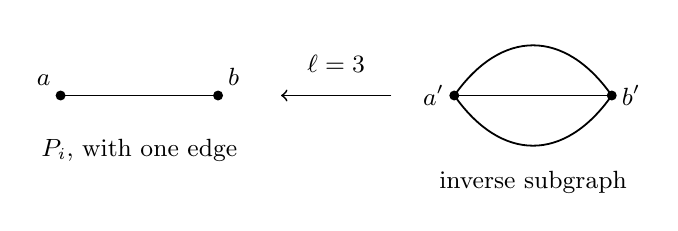
\begin{tikzpicture}[line width=0.65pt, every node/.style={font=\small}]
  \draw (0,0) -- (2,0);
  \fill (0,0) circle (1.8pt) node[above left] {$a$};
  \fill (2,0) circle (1.8pt) node[above right] {$b$};
  \node at (1,-0.7) {$P_i$, with one edge};

  \draw[->] (4.2,0) -- (2.8,0);
  \node at (3.5,0.4) {$\ell=3$};

  \draw (5,0) -- (7,0);
  \draw (5,0) .. controls (5.6,0.85) and (6.4,0.85) .. (7,0);
  \draw (5,0) .. controls (5.6,-0.85) and (6.4,-0.85) .. (7,0);
  \fill (5,0) circle (1.8pt) node[left] {$a'$};
  \fill (7,0) circle (1.8pt) node[right] {$b'$};
  \node at (6,-1.1) {inverse subgraph};
\end{tikzpicture}

\caption{The one-edge case, drawn for $\ell=3$. Connected covers of
the endpoint normalizations give a single vertex $a'$ over $a$ and a
single vertex $b'$ over $b$, whereas the node has three lifts. Any two lifted edges
form a circle. Only this part of the source graph is shown; the actual
paths $P_i$ may have more edges, and their inverse graphs are handled
by the count in the proof.}
\label{fig:path-cycle}
\end{figure}

Let $C$ be the geometric special fibre of the stable model of $Z_0$,
and let $\nu$ denote its normalization. For the constant \'etale
sheaf the normalization sequence is
\[
 0\longrightarrow\mathbb F_\ell\longrightarrow
 \nu_*\mathbb F_\ell\longrightarrow
 \bigoplus_{\text{nodes}}\mathbb F_\ell\longrightarrow0.
\]
The last term is a skyscraper sheaf with vanishing $H^1$, and the
finite normalization has no higher direct images of this sheaf.
Consequently $H^1(C,\mathbb F_\ell)$ surjects onto the product of
the $H^1$ of its normalized components. Each smooth positive-genus
component $D$ admits a nonzero $\mathbb F_\ell$-character. Indeed,
over the algebraically closed residue field, the Kummer sequence gives
$H^1(D,\mu_\ell)=\operatorname{Pic}(D)[\ell]
=\operatorname{Jac}(D)[\ell]$. This group is nonzero by
\cite[Theorem~8.2 and Remark~8.4]{MilneAV}, and a choice
$\mu_\ell\simeq\mathbb F_\ell$ identifies it with the character
group in question. Prescribe such a character at each required
endpoint component and lift this tuple to $H^1(C,\mathbb F_\ell)$.
The resulting torsor is connected: its character is nonzero, and
$\ell$ is prime.

After finite constant extension this torsor is defined on the special
fibre over the residue field. Finite \'etale covers of a proper scheme
over a complete Noetherian local ring are equivalent to those of its
special fibre \cite[Expos\'e~IX, Th\'eor\`eme~1.10]{SGA1}.
Full faithfulness also lifts the action and the torsor identity, giving
a finite \'etale cover of the stable model. Its source is semistable
and normal after every finite constant extension. Its generic fibre
$Z_1$ is geometrically connected: otherwise, after some finite constant
extension, a decomposition of that fibre would extend to open-and-closed
components of the normal model. Each component meets the special fibre
by properness, contradicting its geometric connectedness.

The source model is also stable. On normalized components its map is
finite \'etale, so Riemann--Hurwitz forces any genus-zero source
component to have degree one over a genus-zero component, retaining
at least three node branches. A genus-one component lies over a
genus-one component and retains at least one node branch. Thus no
stabilization can contract the cycles that we now find in its skeleton.

If $P_i$ has $m\ge1$ edges, its inverse graph has $E=m\ell$ edges
and $V\le(m-1)\ell+2$ vertices. Every node has $\ell$ split lifts;
each endpoint has just one vertex above it by the connectedness
imposed on its normalization. Write $c\ge1$ for the number of connected
components of this inverse graph. Then
\[
 b_1=E-V+c\ \ge\ m\ell-((m-1)\ell+2)+1
      =\ell-1>0.
\]
It therefore contains an embedded circle, entirely above $V_i$.

\smallskip\noindent
\emph{Galois refinement preserves the cycles.}
Deck transformations of $Z_0/X$ extend to its stable model. Take the
product over that model of all conjugates of the cyclic cover. After
a finite constant extension, choose a geometric connected component
of its generic fibre and its open-and-closed closure in the normal
product model. On geometric generic fibres this corresponds to the
intersection of the conjugate normal index-$\ell$ subgroups of
$\pi_1(Z_0)$, which is normal in $\pi_1(X)$. The resulting cover
$Z\to X$ is therefore Galois. The chosen component is finite \'etale
and surjective over the model of $Z_1$.

Above a circle with $q$ edges and $q$ vertices, a degree-$e$ finite
\'etale model cover has $eq$ edges and at most $eq$ vertices. Its
nonempty inverse graph consequently satisfies $b_1=E-V+c\ge1$.
The source model is stable by the preceding argument, so its skeleton
contains an embedded circle above each $V_i$, as required.
\end{proof}

\section{Graph characters supported above the disks}

Fix $Z$ as in Proposition~\ref{prop:cycles}, and write
$\tau:Z^{\rm an}\to\Gamma$ for the retraction to its stable skeleton.
Put $U_Z=Z^{\rm an}\times_{X^{\rm an}}U$.

\begin{lemma}\label{lem:graph-character}
For every $i$ there is a connected cyclic finite \'etale cover of $Z$
of degree $p$ which is trivial over all of $U_Z$ and whose restriction
to at least one component above $V_i$ is connected.
\end{lemma}
\begin{proof}
Choose an embedded circle $C_i\subset\Gamma$ lying above $V_i$,
and select one of its edges. We will construct a cyclic graph cover
by gluing sheets only across a cut in this edge. To make its pullback
split over all of $U_Z$, the cut must avoid not just $U_Z$ but its
image under the retraction.

Choose a point $\eta_i$ strictly inside the selected edge at an
irrational position for the normalized valuation. Vertex positions
and edge lengths are rational, so such a point exists. It is of
type three and satisfies
\[
                     \tau^{-1}(\eta_i)=\{\eta_i\}.
\]
Indeed side disks attach only at type-two points, whose coordinates
on this edge have valuation in $\mathbb Q$. Since $\eta_i$ lies
above $V_i$, its singleton retraction fibre misses $U_Z$. Thus
$\tau(U_Z)$ avoids $\eta_i$.

Orient the selected edge and cut it open at $\eta_i$, giving two
new endpoints $\eta_i^-$ and $\eta_i^+$ on its incoming and outgoing
halves. Take $p$ copies of the cut graph, labelled by
$a\in\mathbb F_p$, and identify $\eta_i^-$ in copy $a$ with
$\eta_i^+$ in copy $a+1$. This gives a cyclic graph cover of degree
$p$. Away from $\eta_i$ it is the disjoint union of the $p$ labelled
copies of $\Gamma\setminus\{\eta_i\}$. Traversing $C_i$ in the
selected orientation sends the sheet label $a$ to $a+1$, so the
cover of $C_i$ is connected.

Pull this graph cover back by $\tau$. It splits over the entire
$U_Z$ because $\tau(U_Z)$ misses the cut. On the component above
$V_i$ containing $C_i$, the loop $C_i$ permutes all $p$ sheets
transitively. The restriction to that component, and hence the
pulled-back cover itself, is connected.

It remains to realize this topological cover algebraically. A finite
topological covering of a Berkovich curve obtains an analytic structure
by pulling back the structure sheaf on its locally trivial sheets
\cite[Lemma~2.6]{DeJongCoverings}. The local product
algebras glue by their sheet permutations, giving a coherent finite
\'etale analytic algebra. Proper GAGA algebraizes this algebra,
its unit and multiplication, with their identities preserved by
full faithfulness \cite[Appendix~A, Theorem~A.1(ii)]{GAGA};
\'etaleness is detected after analytification
\cite[Fact~5.1.5]{TemkinAnalytic}. The deck action also algebraizes.
Invariance under the algebraically closed extension $\bar k\subset\Omega$
descends this cover and its action to $\bar k$
\cite[Expos\'e~X, Corollary~1.8]{SGA1}. The resulting cyclic finite
\'etale cover has the two restriction properties just established.
\end{proof}

We have obtained the local nontriviality without sacrificing exterior
splitting. To make it hold on every disk component after one quotient,
we assemble the characters equivariantly.

\section{The stabilizer quotient}

\begin{proof}[Proof of Theorem~\ref{thm:exterior}]
Take the covers of Lemma~\ref{lem:graph-character} for all $i$,
their conjugates under $\Gal(Z/X)$, and a connected component of their
fibre product over $Z$. Call the resulting curve $T$. The intersection
of their kernels in $\pi_1(Z)$ is normal in $\pi_1(X)$, so $T\to X$
is connected, finite \'etale and Galois. Put
\[
 G=\Gal(T/X),\qquad P=\Gal(T/Z).
\]
The group $P$ is elementary abelian of exponent $p$, since it embeds
in the product of the cyclic deck groups. All conjugate covers split
over $U_Z$: each deck transformation of $Z/X$ preserves $U_Z$.
Their composite $P$-cover therefore splits over $U_Z$ as well.

Let $H\subset G$ be the stabilizer of a connected component of the
inverse image of $U$ in $T^{\rm an}$. Splitting over $U_Z$ gives
\begin{equation}\label{eq:disjoint}
                          H\cap P=1.
\end{equation}
Indeed $P$ permutes freely the trivial sheets above each component
of $U_Z$.

For a fixed $i$, choose a component $W$ above $V_i$ in $Z$ on
which the cyclic cover from Lemma~\ref{lem:graph-character} is
connected. Let $A$ be a component above $W$ in $T$, and let
$B\subset G$ be its stabilizer. The stabilizer for $T\to Z$ is
$B\cap P$, so the same fibre calculation as in
Lemma~\ref{lem:components} gives $\deg(A/W)=|B\cap P|$.
The map $A\to W$ factors through the connected restriction of
the chosen cyclic cover. The map to that restriction is surjective:
it is finite \'etale, and its nonzero locally constant rank is
positive everywhere on the connected target. Consequently
$p$ divides $|B\cap P|$.
Lemma~\ref{lem:components} gives transitivity of $G$ on all components
over $V_i$, and $P$ is normal in $G$. Consequently
\begin{equation}\label{eq:nontrivial}
              B\cap P\ne1
 \quad\text{for every such component stabilizer }B.
\end{equation}

Set $Y=T/H$. The two quotients fit into the commutative square
\[
\begin{CD}
 T @>{\text{quotient by }P}>> Z\\
 @V{\text{quotient by }H}VV @VVV\\
 Y @>>> X .
\end{CD}
\]
The curve $Y$ is smooth, proper and connected, and the induced map
$g:Y\to X$ is finite \'etale. We use one component calculation for
both required assertions. Let $D$ be $U$ or one of the $V_i$, and
let $A$ be a component of its inverse image in $T$, with stabilizer
$B\subset G$. The inverse image in $T$ of the image of $A$ in $Y$
is the union of its $H$-translates. This union is open and closed
in the inverse image of $D$, so that image is a connected component
of $g^{-1}(D)$. An
$H$-translate of $A$ is either $A$ or disjoint from it; hence the
image is $A/(B\cap H)$. By Lemma~\ref{lem:components}, its degree
over $D$ is
\[
                         [B:B\cap H].
\]

For the chosen exterior component, $B=H$, so its image has degree
one over $U$. A finite \'etale map of degree one is an isomorphism,
which proves assertion~\textup{(i)}.

Now take any component over $V_i$ in $Y$, and choose a component
above it in $T$ with stabilizer $B$. Put $N=B\cap P$.
By~\eqref{eq:nontrivial}, $N$ is a nontrivial normal $p$-subgroup
of $B$. By~\eqref{eq:disjoint}, $N\cap(B\cap H)=1$. Hence
$B\cap H$ injects into $B/N$, and
\[
 [B:B\cap H]
   =|N|\,[B/N:\operatorname{im}(B\cap H)]
\]
is divisible by $p$. This proves assertion~\textup{(ii)} for every
component above every fixed disk and completes the proof.
\end{proof}

\begingroup
\raggedright
\bibliographystyle{plain}
\bibliography{references}
\endgroup
\end{document}
